\documentclass{article}
\usepackage{graphicx}
\usepackage{amsmath}
\newcommand{\T}{\mathcal{T}}
\begin{document}
We consider the so-called obstacle  problem of finding $u \in K$ such that for all $v \in
K$, 
\begin{align}
&\quad  a(u,v-u)\geq (f,v-u)_{\Omega}   \label{eq:ob-prob}
\end{align}
where
\begin{equation}
  \label{eq:admiss-set}
  K=\{v\in H_0^1\,|\, v\geq \phi \text{ a.e. in }\Omega\},
\end{equation}
\begin{equation}
  a(u,v)=\int_\Omega \nabla u \cdot \nabla v, 
\end{equation}
and 
\begin{equation}
  (f,v)_\Omega=\int_\Omega fv.
\end{equation}

The adaptive numerical method described above is implemented in four steps:
\begin{enumerate}
\item Define an initial triangular mesh, $\T_1$, of $\Omega$.  Use the
  standard finite element method with linear basis to find an
  approximate solution, $u_h^1$, to \eqref{eq:ob-prob}.That is, $u_h^1
  \in K^1$
  satisfies
  \begin{equation}
    \label{eq:fem-obs}
    a(u_h^1,v_h-u_h^1)\geq (f,v_h-u_h^1)_\Omega\, \forall v_h\in K^1
  \end{equation}
where
\begin{align*}
K^1=
\{&v_h\in H^1_0(\Omega)\,|\,v_h(v_i)\geq \phi(v_i) \text{ at all vertices } v_i \text{
  of } \T_1 \\ &\text{ and } \forall K \in T_1,\, v_h|_{K}\in P_1(K)\}.  
\end{align*}


\item Find the free boundary elements of $\T_1$.  An element $K\in
  \T_1$ is said to be a free boundary element if there exist vertices
  $v_1$ and $v_2$ of $K$ such that $u_h^1(v_1)=\phi(v_1)$ and
  $u_h^1(v_2)>\phi(v_2)$. Let the set of free boundary elements of
  $\T_1$ be called $\T_1^F$. 

\item Create a new mesh of $\Omega$, $\T_2$, by refining all the
  elements in $\T_1^F$.  Denote the refinement of $\T_1^F$ as $\T_2^F$,
  let  $h_1^F$ be the maximal edge length in
  $\T_1^F$, let $h_2^F$ be the maximal edge length in $\T_2^F$.   
We choose a \textit{mesh refinement parameter}
  $C$, and  ensure that we refine $T_1^F$ enough times to respect
  the \textit{mesh refinement criteria}
  \begin{equation}
    \label{eq:mesh-refinement-criteria}
    h_2^F\le C \left(h_1^F\right)^{4/3}.
  \end{equation}
In particular, if we use the simple red-green refinement approach for
a two-dimensional mesh, we refine every element of $\T_1^F$ $\left\lceil
\ln\left(C \left(h_1^F\right)^{1/3}\right)\right\rceil$ times. 

The elements $K \notin T_1^F$ are left unrefined,
  except in the case that they must be refined in order to avoid
  hanging nodes.   

\item Use finite element method with quadratic basis on the mesh $\T_2$ to
  find a new approximate solution $u_h^2$ to \eqref{eq:ob-prob}.
  $u_h^2\in K^2$ satisfies

  \begin{equation}
    \label{eq:fem2-obs}
    a(u_h^2,v_h-u_h^2)\geq (f,v_h-u_h^2)_\Omega\, \forall v_h\in K^2
  \end{equation}
where
\begin{align*}
K^2=
\{&v_h\in H^1_0(\Omega)\,|\,v_h(v_i)\geq \phi(v_i) \text{ at all nodes } v_i \text{
  of } \T_2 \\
&\text{ and } \forall K \in T_2,\, v_h|_{K}\in P_2(K)\}.  
\end{align*}
In this context a node of $\T_2$ is defined as any point that is a
vertex of one of the triangles of $\T_2$ or is a midpoint of two such
vertices.  



\end{enumerate}

\section{Numerical Results}
In this section we test the adaptive method on two test cases,
comparing the method with the standard linear and quadratic finite
element method, as well as an adaptive method in which we simply
refine the free boundary mesh $\T_1^F$ one time rather than respecting
the mesh refinement criteria \eqref{eq:mesh-refinement-criteria}.  We
shall refer to the adaptive method which does not respect
\eqref{eq:mesh-refinement-criteria} as the \textit{non-respecting}
adaptive method, and the adaptive method which does respect
\eqref{eq:mesh-refinement-criteria} as the adaptive method. 

\subsection{Example 1}
Let the domain $\Omega=[-1.5,1.5]^2$ and define 
\begin{align}
  &\phi(x)=0 \label{ex1-phi}\\
  &f(x)=-2\label{ex1-f}\\
  &u_0(r)=\frac{r^2}{2}-\ln(r)-1/2 \label{ex1-u0}.
\end{align}
where $r=\sqrt{x_1^2+x_2^2}$.

With these choices of parameters the exact solution to
\eqref{eq:ob-prob}--\eqref{eq:admiss-set} is
\begin{equation}
  \label{eq:ex1-u}
u(r)=  \begin{cases}
  0 &\text{ if } r<1\\
  \frac{r^2}{2}-\ln(r)-1/2 & \text{ otherwise.}
\end{cases}
\end{equation}

In the numerical examples we choose the mesh refinement parameter $C=10$.  

In Figures \ref{fig:example1-error}--\ref{fig:example1-time} we compare the
accuracy of each of the four numerical methods, as well as the time
required to compute each solution.  We can see that the adaptive
method outperforms the other methods in both regards.  As expected,
the non-respecting adaptive method  begins to lose accuracy compared
the adaptive method as the mesh size becomes small. 

We report the same results in tabular form in Tables
\ref{tab:example1-linear} -- \ref{tab:example1-adaptive}.  In
addition, for each numerical method we
approximate the order of convergence by comparing the error achieved
by the $i^{th}$ approximation to the error achieved by the first
approximation.  In particular, let $N_i$ denote the number of degrees of
freedom corresponding to the $i^{th}$ approximation. Let $h_i$ denote the
largest edge length from the mesh $\T^1_i$, and define $E_i$ as the
$H^1(\Omega)$ error achieved by approximation $i$. We estimate the
order of convergence in terms of $N$ for the method by $p\approx
\frac{\log(E_i/E_1)}{\log(N_i/N_1)}$. We estimate the order of
convergence in terms of $h$ via $p\approx
\frac{\log(E_i/E_1)}{\log(h_i/h_1)}$.  As a second  estimate of
convergence order in terms of $h$ we find the least-squares solution
to the system of equations $\ln E_i=p\ln h_i +c$ and report the value
of $p$, a second estimate of the convergence order in terms of $N$ is
computed similarly. 
In Tables
\ref{tab:example1-linear} -- \ref{tab:example1-adaptive} we can see
each method tending toward its expected order of convergence. 


\begin{figure}
\includegraphics[width=4in]{example1/Error.pdf}
\caption{Degrees of freedom vs. $H^1$ error for Example 1.}
\label{fig:example1-error}
\end{figure}

\begin{figure}
\includegraphics[width=4in]{example1/ErrorH.pdf}
\caption{Mesh size vs. $H^1$ error for Example 1.}
\label{fig:example1-herror}
\end{figure}


\begin{figure}
\includegraphics[width=4in]{example1/ComputingTime.pdf}
\caption{Solution time (s) vs. $H^1$ error for Example 1.}
\label{fig:example1-time}
\end{figure}



\begin{table}
\begin{tabular}{|r|r|r|r|r|r|}
\hline
$N$&$h$&$H^1$ Error&$N$ Conv. Rate &$h$ Conv. Rate&Comp. Time (s)\\ 
\hline
\hline
17&1.677e+00&1.207e+00&-&-&0\\ 
31&1.008e+00&7.486e-01&-7.945e-01&9.372e-01&9.372e-01\\ 
101&5.252e-01&3.527e-01&-6.902e-01&1.059e+00&1.059e+00\\ 
366&2.650e-01&1.800e-01&-6.198e-01&1.031e+00&1.031e+00\\ 
1385&1.325e-01&9.085e-02&-5.878e-01&1.019e+00&1.019e+00\\ 
5308&6.629e-02&4.588e-02&-5.692e-01&1.012e+00&1.012e+00\\ 
20958&3.315e-02&2.292e-02&-5.569e-01&1.010e+00&1.010e+00\\ 
83087&1.657e-02&1.146e-02&-5.482e-01&1.009e+00&1.009e+00\\ 
330653&8.286e-03&5.749e-03&-5.414e-01&1.007e+00&1.007e+00\\
\hline 
Best Fit&&&-5.308e-01&1.007e+00&\\ 
\hline
\end{tabular}
\caption{Results for linear method in Example 1.}
\label{tab:example1-linear}
\end{table}


\begin{table}
\begin{tabular}{|r|r|r|r|r|r|}
\hline
$N$&$h$&$H^1$ Error&$N$ Conv. Rate &$h$ Conv. Rate&Comp. Time (s)\\ 
\hline
\hline
49&1.677e+00&5.900e-01&-&-&0\\ 
105&1.008e+00&1.390e-01&-1.897e+00&2.839e+00&2.839e+00\\ 
369&5.252e-01&7.419e-02&-1.027e+00&1.786e+00&1.786e+00\\ 
1397&2.650e-01&2.064e-02&-1.001e+00&1.817e+00&1.817e+00\\ 
5409&1.325e-01&7.199e-03&-9.367e-01&1.736e+00&1.736e+00\\ 
20973&6.629e-02&2.639e-03&-8.928e-01&1.674e+00&1.674e+00\\ 
83317&3.315e-02&9.073e-04&-8.708e-01&1.651e+00&1.651e+00\\ 
331319&1.657e-02&3.206e-04&-8.524e-01&1.628e+00&1.628e+00\\ 
1320561&8.286e-03&1.122e-04&-8.398e-01&1.613e+00&1.613e+00\\
\hline 
Best Fit&&&-8.037e-01&1.563e+00&\\ 
\hline
\end{tabular}
\caption{Results for quadratic method in Example 1.}
\label{tab:example1-quadratic}
\end{table}



\begin{table}
\begin{tabular}{|r|r|r|r|r|r|}
\hline
$N$&$h$&$H^1$ Error&$N$ Conv. Rate &$h$ Conv. Rate&Comp. Time (s)\\ 
\hline
\hline
137&1.677e+00&2.050e-01&-&-&0\\ 
320&1.008e+00&6.373e-02&-1.377e+00&2.295e+00&2.295e+00\\ 
815&5.252e-01&2.825e-02&-1.111e+00&1.707e+00&1.707e+00\\ 
2413&2.650e-01&8.183e-03&-1.123e+00&1.746e+00&1.746e+00\\ 
7185&1.325e-01&3.106e-03&-1.058e+00&1.651e+00&1.651e+00\\ 
24593&6.629e-02&1.190e-03&-9.921e-01&1.594e+00&1.594e+00\\ 
90277&3.315e-02&4.474e-04&-9.441e-01&1.562e+00&1.562e+00\\ 
345815&1.657e-02&1.512e-04&-9.207e-01&1.562e+00&1.562e+00\\ 
1349265&8.286e-03&5.192e-05&-9.006e-01&1.559e+00&1.559e+00\\
\hline 
Best Fit&&&-8.796e-01&1.517e+00&\\ 
\hline
\end{tabular}
\caption{Results for adaptive (non-respecting) method in Example 1.}
\label{tab:example1-adaptiveno43}
\end{table}

\begin{table}
\begin{tabular}{|r|r|r|r|r|r|}
\hline
$N$&$h$&$H^1$ Error&$N$ Conv. Rate &$h$ Conv. Rate&Comp. Time (s)\\ 
\hline
\hline
137&1.677e+00&2.050e-01&-&-&0\\ 
320&1.008e+00&6.373e-02&-1.377e+00&2.295e+00&2.295e+00\\ 
815&5.252e-01&2.825e-02&-1.111e+00&1.707e+00&1.707e+00\\ 
2413&2.650e-01&8.183e-03&-1.123e+00&1.746e+00&1.746e+00\\ 
13725&1.325e-01&1.481e-03&-1.070e+00&1.943e+00&1.943e+00\\ 
80125&6.629e-02&3.434e-04&-1.003e+00&1.979e+00&1.979e+00\\ 
196377&3.315e-02&1.099e-04&-1.036e+00&1.919e+00&1.919e+00\\ 
1147579&1.657e-02&2.388e-05&-1.003e+00&1.962e+00&1.962e+00\\
\hline 
Best Fit&&&-9.897e-01&1.958e+00&\\ 
\hline
\end{tabular}
\caption{Results for adaptive (respecting) method in Example 1.}
\label{tab:example1-adaptive}
\end{table}


\subsection{Example 2}
As in Example 1, let the domain be $\Omega=[-1.5,1.5]^2$. Define the parameters
\begin{align}
  &\phi(x)=0, \label{ex2-phi}\\
  &f(r)=\begin{cases}\sqrt{1-r^2}&\text{ if } r<1 \\
                                  0&\text{otherwise}\end{cases},\label{ex2-f}\\
  &r^*=0.6979651482,\\
  &u_0(r)=-\left(r^*\right)^2\frac{\ln(r/2)}{\sqrt{1-\left(r^*\right)^2}} \label{ex2-u0}.
\end{align}

where $r=\sqrt{x_1^2+x_2^2}$.

With these choices of parameters the exact solution to
\eqref{eq:ob-prob}--\eqref{eq:admiss-set} is
\begin{equation}
  \label{eq:ex1-u}
u(r)=  \begin{cases}
  \sqrt{1-r^2} &\text{ if } r<r^*\\
  -\left(r^*\right)^2\frac{\ln(r/2)}{\sqrt{1-\left(r^*\right)^2}} & \text{ otherwise.}
\end{cases}
\end{equation}

Again we choose the mesh refinement parameter $C=10$.  

Figures \ref{fig:example2-error} and \ref{fig:example2-time} compare
the error and solution time in each of the methods.  Once again the
adaptive method outperforms the other methods.  

Tables \ref{tab:example2-linear}--~\ref{tab:example2-adaptive} provide
the same data as the figures in tabular form, and attempt to estimate
the convergence rate of each method. Again, the adaptive method
converges at a rate near $N^{-1}$, as predicted.  


\begin{figure}
\includegraphics[width=4in]{example2/Error.pdf}
\caption{Degrees of freedom vs. $H^1$ error for Example 2.}
\label{fig:example2-error}
\end{figure}

\begin{figure}
\includegraphics[width=4in]{example2/ErrorH.pdf}
\caption{Mesh size vs. $H^1$ error for Example 2.}
\label{fig:example2-herror}
\end{figure}


\begin{figure}
\includegraphics[width=4in]{example2/ComputingTime.pdf}
\caption{Solution time (s) vs. $H^1$ error for Example 2.}
\label{fig:example2-time}
\end{figure}



\begin{table}
\begin{tabular}{|r|r|r|r|r|r|}
\hline
$N$&$h$&$H^1$ Error&$N$ Conv. Rate &$h$ Conv. Rate&Comp. Time (s)\\ 
\hline
\hline
17&1.677e+00&5.765e-01&-&-&0\\ 
31&1.008e+00&7.005e-01&3.244e-01&-3.827e-01&-3.827e-01\\ 
101&5.252e-01&3.386e-01&-2.985e-01&4.582e-01&4.582e-01\\ 
366&2.650e-01&1.666e-01&-4.043e-01&6.727e-01&6.727e-01\\ 
1385&1.325e-01&8.278e-02&-4.410e-01&7.646e-01&7.646e-01\\ 
5308&6.629e-02&4.216e-02&-4.553e-01&8.095e-01&8.095e-01\\ 
20958&3.315e-02&2.124e-02&-4.638e-01&8.412e-01&8.412e-01\\ 
83087&1.657e-02&1.065e-02&-4.699e-01&8.646e-01&8.646e-01\\ 
330653&8.286e-03&5.327e-03&-4.743e-01&8.821e-01&8.821e-01\\ 
\hline
Best Fit&&&-5.014e-01&9.470e-01&\\ 
\hline
\end{tabular}
\caption{Results for linear method in Example 2}
\label{tab:example2-linear}
\end{table}

\begin{table}
\begin{tabular}{|r|r|r|r|r|r|}
\hline
$N$&$h$&$H^1$ Error&$N$ Conv. Rate &$h$ Conv. Rate&Comp. Time (s)\\ 
\hline
\hline
49&1.677e+00&6.289e-01&-&-&0\\ 
105&1.008e+00&1.520e-01&-1.864e+00&2.789e+00&2.789e+00\\ 
369&5.252e-01&7.797e-02&-1.034e+00&1.798e+00&1.798e+00\\ 
1397&2.650e-01&3.447e-02&-8.668e-01&1.574e+00&1.574e+00\\ 
5409&1.325e-01&1.225e-02&-8.372e-01&1.552e+00&1.552e+00\\ 
20973&6.629e-02&4.679e-03&-8.088e-01&1.517e+00&1.517e+00\\ 
83317&3.315e-02&1.549e-03&-8.075e-01&1.531e+00&1.531e+00\\ 
331319&1.657e-02&5.615e-04&-7.961e-01&1.521e+00&1.521e+00\\ 
1320561&8.286e-03&1.973e-04&-7.908e-01&1.519e+00&1.519e+00\\ 
\hline
Best Fit&&&-7.477e-01&1.454e+00&\\ 
\hline
\end{tabular}
\caption{Results for quadratic method in Example 2.}
\label{tab:example2-quadratic}
\end{table}

\begin{table}
\begin{tabular}{|r|r|r|r|r|r|}
\hline
$N$&$h$&$H^1$ Error&$N$ Conv. Rate &$h$ Conv. Rate&Comp. Time (s)\\ 
\hline
\hline
137&1.677e+00&1.459e-01&-&-&0\\ 
314&1.008e+00&9.188e-02&-5.573e-01&9.076e-01&9.076e-01\\ 
737&5.252e-01&4.031e-02&-7.643e-01&1.108e+00&1.108e+00\\ 
2053&2.650e-01&1.582e-02&-8.207e-01&1.204e+00&1.204e+00\\ 
6693&1.325e-01&5.669e-03&-8.351e-01&1.280e+00&1.280e+00\\ 
23485&6.629e-02&2.136e-03&-8.211e-01&1.307e+00&1.307e+00\\ 
88285&3.315e-02&6.834e-04&-8.292e-01&1.367e+00&1.367e+00\\ 
341451&1.657e-02&2.500e-04&-8.144e-01&1.379e+00&1.379e+00\\ 
1340053&8.286e-03&8.805e-05&-8.067e-01&1.396e+00&1.396e+00\\ 
\hline
Best Fit&&&-8.239e-01&1.423e+00&\\ 
\hline
\end{tabular}
\caption{Results for adaptive (non-respecting) method in Example 2.}
\label{tab:example2-adaptiveno43}
\end{table}

\begin{table}
\begin{tabular}{|r|r|r|r|r|r|}
\hline
$N$&$h$&$H^1$ Error&$N$ Conv. Rate &$h$ Conv. Rate&Comp. Time (s)\\ 
\hline
\hline
137&1.677e+00&1.459e-01&-&-&0\\ 
314&1.008e+00&9.188e-02&-5.573e-01&9.076e-01&9.076e-01\\ 
737&5.252e-01&4.031e-02&-7.643e-01&1.108e+00&1.108e+00\\ 
2053&2.650e-01&1.582e-02&-8.207e-01&1.204e+00&1.204e+00\\ 
11429&1.325e-01&2.423e-03&-9.263e-01&1.615e+00&1.615e+00\\ 
61305&6.629e-02&5.707e-04&-9.083e-01&1.716e+00&1.716e+00\\ 
164273&3.315e-02&1.874e-04&-9.391e-01&1.697e+00&1.697e+00\\ 
897539&1.657e-02&4.314e-05&-9.247e-01&1.760e+00&1.760e+00\\ 
5366497&8.286e-03&1.488e-05&-8.690e-01&1.731e+00&1.731e+00\\ 
\hline
Best Fit&&&-9.172e-01&1.828e+00&\\ 
\hline
\end{tabular}
\caption{Results for adaptive (respecting) method in Example 2.}
\label{tab:example2-adaptive}
\end{table}



\end{document}
